% 第 10 章：例：tetration 与其他族
\providecommand{\STreg}{\mathcal{ST}}          % Shell--Thron 区
\providecommand{\Uup}{\mathcal U^{+}}          % 上半 Shell--Thron 区
\providecommand{\Eup}{\mathcal E^{+}}          % 上半平面中 Shell--Thron 区的外部
\providecommand{\Ftr}{F^{\mathrm{tr}}}         % 输运族

\chapter{例：tetration 与其他族}\label{ch:examples}

前九章在一般实鞍结开折的设定下建立了理论。本章把它用到具体的族上。
第一个例子是 tetration，即方程
\begin{equation}\label{ch10:eq:tetration}
  F(z+1)=b^{F(z)},\qquad F(0)=1 .
\end{equation}
它是本理论的出发点：缝合解、汇流与一阶项最初都是为它证明的~\cite{KneserPaper}。
它也是目前唯一完成了\textbf{整体延拓}的例子：Kneser 在 1950 年对 $b=\ee$ 给出、并可逐字推广到每个实底数 $b>\eta=\ee^{1/\ee}$ 的
构造，所得的解可以沿底数延拓，绕过尖点 $\eta$，并且在整个上半 $b$ 平面上单值。
这两个整体结果依赖指数函数的整体几何（Shell--Thron 区的形状，$b=0,1$ 两个奇点），
不属于一般理论。它们的证明很长（论文第 10 节约 2300 行，外加区间证书），
本章只给出精确陈述、证明的结构和关键引理，并逐条指出论文中的出处。

本章后半部分讨论另外三个族 $w^2+c$、$v-\sin v+c$ 和 $w+(w^2-c)\ee^w$。
一般理论（第 5--9 章）对它们直接成立；整体延拓只对 $w^2+c$ 有一份单独的证明稿，
另外两个族只有数值。

\begin{goals}
\item tetration 是满足 (H1)--(H5) 的实鞍结开折，$a_2=\tfrac12$，$\gamma=1$，$\rho=\tfrac13$；本章列出它的全部常数。
\item Kneser 的构造：两个共轭不动点之间的弦、弦的像、粘合成柱面、共形单值化。
\item 底数平面的几何：Shell--Thron 区、尖点 $\eta$、中性弧 $\beta(\alpha)$、端点 $\ee^{-\ee}$、奇点 $0$ 与 $1$。
\item \cref{thm:cusp}：Kneser 解绕过尖点，跨过中性弧，边界值等于缝合解 $\Ksew_b$；证明的结构是倾斜初始区域加 Ahlfors--Bers 定理。
\item \cref{thm:upper-half-plane}：在整个上半 $b$ 平面单值全纯（计算机辅助）；按 Paulsen 的定义理解，它就是 Paulsen 的族。
\item 其他三个族：哪些结论由一般理论推出，哪些是单独证明的，哪些只是数值。
\end{goals}

本章的状态标记与理论文档一致：「已证」指纸面证明；「证·机」指纸面证明加区间算术证书；
「数值」指数值证据；「猜想」指猜想。

% ======================================================================
\section{tetration 作为鞍结开折}\label{ch10:sec:unfolding}

记 $E_b(w)=b^w=\ee^{w\log b}$。本节只考虑实底数 $1<b<\eta$ 附近，$\log b$ 取实值。

\begin{lemma}[乘子参数化]\label{ch10:lem:param}
设 $L$ 是 $E_b$ 的不动点，乘子 $\lambda=L\log b$。则
\[
  L=\ee^{\lambda},\qquad \log b=\lambda\ee^{-\lambda}.
\]
函数 $\lambda\mapsto\lambda\ee^{-\lambda}$ 在 $(0,1)$ 上递增，在 $(1,\infty)$ 上递减，最大值 $\ee^{-1}=\log\eta$。
因此吸引不动点的乘子 $\lambda_1\in(0,1)$ 与排斥不动点的乘子 $\lambda_2\in(1,\infty)$ 各自参数化 $(1,\eta)$，
两支在 $b=\eta$ 处相遇。
\end{lemma}

\begin{proof}
由 $L=b^L$ 得 $\log L=L\log b=\lambda$。其余是 $(\lambda\ee^{-\lambda})'=(1-\lambda)\ee^{-\lambda}$ 的符号。
\end{proof}

在以 $w^*=\ee$ 为中心的仿射坐标 $w=w^*+\ee\,u=\ee(1+u)$（伸缩因子取 $\ee$，与论文一致）中，令
\begin{equation}\label{ch10:eq:s}
  s=1-\ee\log b ,
\end{equation}
则 $E_b$ 变为
\begin{equation}\label{ch10:eq:fs}
  f_s(u)=\ee^{(1-s)(1+u)-1}-1=\ee^{\,u-s(1+u)}-1 .
\end{equation}
$s>0$ 对应 $b<\eta$。

\begin{proposition}[tetration 的开折数据]\label{ch10:prop:data}
族~\eqref{ch10:eq:fs} 满足 \cref{def:unfolding} 的 (H1)--(H5)，数据如下。
\begin{enumerate}
\item 芽 $g(u)=f_0(u)=\ee^u-1=u+\tfrac12u^2+\tfrac16u^3+\cdots$，所以 $a_2=\tfrac12$，$a_3=\tfrac16$，
  $\rho=1-a_3/a_2^2=\tfrac13$。形式 Abel 函数是 $\alpha(u)=-2/u+\tfrac13\log(-u)+O(u)$。
\item 开折方向 $X=-\partial_sf_s|_{s=0}=(1+u)\ee^u$，横截性 $\gamma=X(0)=1$。
\item 基点 $w_0=1$，即 $\ustar=\ee^{-1}-1$；它在 $g$ 的直接吸引花瓣中。
\item $B_1\neq0$（\cref{prop:B1-nonzero}）。
\end{enumerate}
\end{proposition}

\begin{proof}
(H1)：$f_s(u)$ 对 $u$ 整，对 $s$ 整，实对实。(H2)、(H3) 是 (1)、(2) 的直接计算。
(H4)：对 $u<0$ 有 $u<\ee^u-1<0$，所以负实轴上的轨道单调增加并趋于 $0$，$g$ 在 $[\ustar,0)$ 上递增且 $g(u)>u$。
(H5) 是 \cref{prop:B1-nonzero}：$\ee^u-1$ 没有临界点，只有一个有限奇异值 $-1$（沿负实轴的渐近值），
因此属于 Chéritat 的单奇值类~\cite[命题~2.4]{KneserPaper}。
\end{proof}

开折方向与平移方向只差一个无穷小共轭：
\begin{equation}\label{ch10:eq:cohomologous}
  X-1=\Lop(-2-u),\qquad \Lop\varphi=\varphi\circ g-g'\varphi .
\end{equation}
事实上 $\Lop(-2-u)=-2-(\ee^u-1)-\ee^u(-2-u)=(1+u)\ee^u-1$。
由 \cref{cor:variation}，tetration 的一阶系数的实部等于平移开折 $g-s$ 的一阶系数的实部：
\begin{equation}\label{ch10:eq:retr}
  \Rea\kappa^{(n)}=\Rea\ktr^{(n)}(\ee^u-1).
\end{equation}

\begin{proposition}[尺度]\label{ch10:prop:scale}
记 $\varepsilon=1-\lambda_1$。当 $b\to\eta^-$ 时，
\[
  \varepsilon=\sqrt{2\ee(\log\eta-\log b)}\,(1+O(\varepsilon)),\qquad
  p=-\log\lambda_1\cdot\log\lambda_2=2s+\tfrac{10}{9}s^2+O(s^3),
\]
\[
  \Lam=\exp\Bigl(-\frac{C_\eta}{\sqrt{\eta-b}}\,(1+o(1))\Bigr),\qquad
  C_\eta=\frac{4\pi^2}{\sqrt{2\ee^{1-1/\ee}}}=20.3508\ldots .
\]
\end{proposition}

\begin{proof}
$\lambda\ee^{-\lambda}=\ee^{-1}(1-\tfrac12\varepsilon^2-\tfrac13\varepsilon^3+O(\varepsilon^4))$ 给出第一式。
由 \cref{prop:scales}，$|\log\lambda_1|=2\sqrt{a_2\gamma s}(1+O(\sqrt s))=\sqrt{2s}(1+O(\sqrt s))$，$p=4a_2\gamma s+O(s^2)=2s+O(s^2)$；
$s^2$ 的系数 $\tfrac{10}9$ 由 $\lambda_{1,2}$ 关于 $\varepsilon$ 的展开直接算出（习题~\ref{ch10:ex:p}）。
又 $s=1-\ee\log b=\ee(\log\eta-\log b)\sim\ee^{1-1/\ee}(\eta-b)$，代入
$\Lam=\exp(4\pi^2/\log\lambda_1)=\exp(-2\pi^2/\sqrt{s/2}\,(1+o(1)))$ 即得 $C_\eta$。
\end{proof}

\begin{example}[tetration 的常数]\label{ch10:ex:constants}
下表汇集 tetration 的全部常数。数值来源如下。
\begin{itemize}\sloppy
\item 区间包络：论文附录 A.5 的证书 \texttt{certify\_horn\_coefficients.py} 与 \texttt{certify\_parabolic\_a.py}（python-flint/Arb）。
\item $\kappa^{(1)}$：论文定理 5.6 的抛物级数；其实部由 \texttt{kappa\_variation.py} 独立复核。
\item $C_\eta$：由 \texttt{figures/fig10\_shell\_thron.py} 打印。
\end{itemize}
\begin{center}\footnotesize
\begin{tabular}{lll}
\toprule
量 & 值 & 状态\\
\midrule
$a_2,\ a_3,\ \rho,\ \gamma$ & $\tfrac12,\ \tfrac16,\ \tfrac13,\ 1$ & 精确\\
$X$ & $(1+u)\ee^u$，$X-1=\Lop(-2-u)$ & 精确\\
$\ustar$ & $\ee^{-1}-1$ & 精确\\
$a=\Phiatt(\ustar)$ & $3.02929721441803609892499\ldots$ & 证·机\\
$|B_1|$ & $0.089058436412213331563\ldots$ & 证·机\\
$B_2/B_1^2$ & $-0.0253204931+1.5742190652\,\ii$ & 证·机（10 位）\\
$\arg B_1+2\pi a\pmod{2\pi}$ & $1.5865330757\ldots$ & 数值\\
$C_\eta$ & $20.3508008134\ldots$ & 精确公式\\
$\kappa^{(1)}$ & $-0.010199006345897402441-0.013250956182506712250\,\ii$ & 数值（级数求和）\\
$\kappa^{(1)}_2$ & $-7.88992074991511334\cdot10^{-5}+3.6554727325799459\cdot10^{-4}\,\ii$ & 数值\\
\bottomrule
\end{tabular}
\end{center}
$\kappa^{(1)}$ 与 $b<\eta$ 一侧的拟合在拟合的全部 11 位上一致，$\kappa^{(1)}_2$ 在第 6 位上相差不超过一个单位。
由~\eqref{ch10:eq:retr}，$\Rea\kappa^{(1)}=-0.0101990063458974$ 也是 $\ee^u-1$ 的平移开折的值；
第 9 章的变分公式数值检验（\cref{thm:variation}）正是用这一行做的。
\end{example}

\begin{remark}[记号]\label{ch10:rem:notation}
论文~\cite{KneserPaper} 把吸引正则解记为 $\mathcal R_b$，并用 $F(0)=1$ 归一化；在 $u$ 坐标中这就是
本书的 $R$ 以 $R^{-1}(w_0)=0$ 归一化（\cref{def:regular-solution}）。
论文中的 $\mathcal L=\log b$、$g_\theta$、$X$（商曲面）、$\Lambda$（外部乘子区域）等记号与本书冲突，下文分别改写为 $\log b$、$k_\theta$、$\Sigma$、$\mathcal V$。
\end{remark}

% ======================================================================
\section{Kneser 1950 年的构造}\label{ch10:sec:kneser}

对实底数 $b>\eta$，$E_b$ 在实轴上没有不动点：$E_b(x)-x$ 在 $x\to\pm\infty$ 时为正，且没有实零点。
所以实轴上没有可以作为 Koenigs 坐标中心的点。Kneser~\cite{Kneser1950} 的想法是使用
离实轴最近的一对复共轭不动点。

\subsection{两个共轭不动点}

设 $b>\eta$。由 \cref{ch10:lem:param}，不动点 $L$ 满足 $L=\ee^\lambda$，$\lambda\ee^{-\lambda}=\log b>\ee^{-1}$。
取主不动点对 $L_\pm$，由 $0<\Ima(L_+\log b)<\pi$ 刻画，$L_-=\overline{L_+}$。写
$\theta=\Ima(L_+\log b)\in(0,\pi)$，则乘子 $\lambda_+=L_+\log b$ 的实部是 $\theta\cot\theta$（习题~\ref{ch10:ex:exterior}），即
\begin{equation}\label{ch10:eq:exterior-multiplier}
  \lambda_\pm=\theta\cot\theta\pm\ii\theta,\qquad |\lambda_\pm|=\frac{\theta}{\sin\theta}>1 .
\end{equation}
两个不动点都是排斥的，而且乘子不是实数。

\subsection{初始区域}

令 $u_b=\Rea L_+$，$v_b=\Ima L_+>0$，$\gamma_b(t)=u_b+\ii v_bt$（$-1\le t\le1$）是连接 $L_-$ 与 $L_+$ 的竖直弦。
记 $r_b=|L_+|$，$\theta_b=v_b\log b$。直接计算得
\[
  E_b(\gamma_b(t))=r_b\,\ee^{\ii\theta_bt},
\]
即弦的像是以原点为心、半径 $r_b$ 的圆弧。弦与像弧只在 $L_\pm$ 处相交，围出
\begin{equation}\label{ch10:eq:initial-region}
  H_b=\{\Rea w\ge u_b,\ |w|\le r_b\}\setminus\{L_+,L_-\} .
\end{equation}
这就是 Kneser 的\textbf{初始区域}（initial region）；Trappmann 与 Kouznetsov 用它刻画 Kneser 解~\cite{TrappmannKouznetsov2011}。

把弦上的点 $w$ 与像弧上的点 $E_b(w)$ 粘合，得到一个 Riemann 曲面 $\Sigma_b$。
它是一个两端开口的柱面，两端对应 $L_+$ 与 $L_-$。在 $L_\pm$ 附近，$E_b$ 由 Koenigs 坐标 $\sigma_\pm$ 线性化
（\cref{thm:koenigs}；两个不动点都是双曲的），
\[
  \exp\Bigl(\frac{2\pi\ii\log\sigma_\pm}{\log\lambda_\pm}\Bigr)
\]
是粘合后一端的穿孔坐标。所以两端都是穿孔圆盘，$\Sigma_b\cong\C^*$。
取单值化 $Z:\Sigma_b\to\C^*$，把 $L_+$ 端送到 $0$，令 $z=(2\pi\ii)^{-1}\log Z$。
跨过粘合线时 $z$ 增加 $1$，所以 $z$ 的逆映射沿 $F(z+1)=E_b(F(z))$ 延拓为一个超函数（superfunction）。
最后用实轴上的轨道把 $z$ 归一化为 $z(1)=0$。由实对称性（共轭交换两端并固定标记点 $1$），$z$ 在正实轴上取实值并严格递增。
所得的解记为 $\Kkn_b$，称为 \textbf{Kneser 解}（Kneser's solution）。

\begin{remark}[Kneser 的原始论证]\label{ch10:rem:kneser-original}
Kneser 原文处理 $b=\ee$（目标是半指数 $\vartheta(\vartheta(x))=\ee^x$），步骤是：
在不动点 $c\approx0.318+1.337\ii$ 处，$c$ 对 $\log$ 是吸引的（$|1/c|<1$），用 Koenigs 定理得 $\chi$，$\chi(\ee^z)=c\chi(z)$；
取对数 $\omega=\log\chi$，得 $\omega(\ee^z)=\omega(z)+\Log c=\omega(z)+c$（$c$ 是 $\exp$ 的不动点且 $|\Ima c|<\pi$，所以 $\Log c=c$），指数函数变成沿复方向 $c$ 的平移；
实轴在 $\omega$ 平面中的像是一条 $c$-周期曲线，它上方的区域模去 $c$-平移是一个半柱面；
再用共形映射把它单值化为模 $1$ 的上半柱面，并使实轴的像回到实轴。
上下两侧用反射拼接，就得到一个实解析 Abel 函数 $\Psi$，$\Psi(\ee^x)=\Psi(x)+1$。
初始区域的说法与这个说法等价：两者都是在构造同一个柱面的单值化。
初始区域的说法更便于讨论参数依赖，下文只用它。
\end{remark}

\subsection{对实底数的解析依赖}

Kneser 的构造对每个实 $b>\eta$ 单独进行。为了沿底数延拓，需要先知道它在实轴上关于 $b$ 实解析。
\cite{Paulsen2019} 的命题 3 断言了这一点，但没有单独的参数依赖证明。下面的命题给出证明。

\begin{proposition}[外侧实射线上的局部解析性；{\cite[命题~10.11]{KneserPaper}}]\label{ch10:prop:exterior-real}
对每个实 $b_0>\eta$，Kneser 解 $\Kkn_b$ 在 $\Delta\times W$ 上有关于 $(b,z)$ 联合全纯的延拓，
其中 $\Delta$ 是 $b_0$ 的复圆盘，$W$ 是 $[0,1]$ 的复邻域。这些局部延拓在重叠处一致。
\end{proposition}

\begin{proof}[证明思路]
$L_\pm(b)$ 是单不动点，对 $b$ 全纯，所以弦和像弧对 $b$ 全纯地运动；缩小 $\Delta$ 后它们仍然只在端点相交
（端点处切线不同，因为乘子不是实数）。粘合得到柱面的全纯族；两端用依赖参数的 Koenigs 坐标填上，
得到紧亏格零曲面的真全纯淹没。再加上由 $w=1$ 给出的全纯截面（实轨道把 $1$ 搬进初始区域），
就有三个互不相交的全纯截面。Fischer--Grauert 局部平凡性~\cite{FischerGrauert1965}
加上三点 Möbius 归一化，给出联合全纯的坐标 $q_b$。取对数提升并求逆即得。
在实底数处，所得的逆就是 Kneser 的实归一化解，这一点用 \cite[定理~1、定理~5]{TrappmannKouznetsov2011} 的初始区域判据核对。
\end{proof}

% ======================================================================
\section{底数平面}\label{ch10:sec:base-plane}

\subsection{Shell--Thron 区}

令 $b(\lambda)=\exp(\lambda\ee^{-\lambda})$。由 \cref{ch10:lem:param}，若 $E_b$ 有乘子为 $\lambda$ 的不动点，则 $b=b(\lambda)$。

\begin{lemma}[全局参数；{\cite[引理~10.17]{KneserPaper}}]\label{ch10:lem:global-param}
$b(\lambda)$ 在单位圆盘 $\D$ 上单射；$E_{b(\lambda)}$ 有不动点 $\ee^\lambda$，乘子为 $\lambda$；
$b(\D)$ 恰是使 $E_b$ 有吸引不动点的底数集合。$\Uup:=b(\D\cap\HH)$ 含于上半平面且单连通。
\end{lemma}

\begin{proof}
令 $\phi(\lambda)=\lambda\ee^{-\lambda}$。在 $\D$ 上 $\Rea(\lambda\phi'/\phi)=\Rea(1-\lambda)>0$，所以 $\phi$ 是星形单叶的。
又 $|\phi|<\ee<\pi$，故 $\ee^{\phi(\lambda_1)}=\ee^{\phi(\lambda_2)}$ 推出 $\phi(\lambda_1)=\phi(\lambda_2)$，从而 $b$ 单射。
若 $E_b$ 的不动点 $L$ 的乘子 $\lambda=L\log b$ 满足 $|\lambda|<1$，则 $\log b=\phi(\lambda)$（\cref{ch10:lem:param}）。
由对称性和单射性，$\phi$ 把上半圆盘映入 $\{\Ima>0\}$；又 $|\Ima\phi|<\pi$，所以 $\Ima b>0$。
单连通区域的单射像是单连通的。
\end{proof}

$b(\D)$ 的闭包称为 \textbf{Shell--Thron 区}（Shell--Thron region），记为 $\overline{\STreg}$。
它得名于无穷幂塔 $b^{b^{b^{\cdots}}}$ 的收敛问题：Thron~\cite{Thron1957} 与 Shell~\cite{Shell1962} 证明了幂塔在这个区域的内部收敛（边界点的情形更细致）；本书不用这个事实。
它的边界是曲线
\begin{equation}\label{ch10:eq:beta}
  \beta(\alpha)=\exp\bigl(\ee^{\ii\alpha}\ee^{-\ee^{\ii\alpha}}\bigr),\qquad -\pi\le\alpha\le\pi ,
\end{equation}
即乘子为 $\ee^{\ii\alpha}$ 的中性不动点出现的底数。$\{\beta(\alpha):0<\alpha<\pi\}$ 称为\textbf{上中性弧}。

\begin{figure}[ht]
\centering
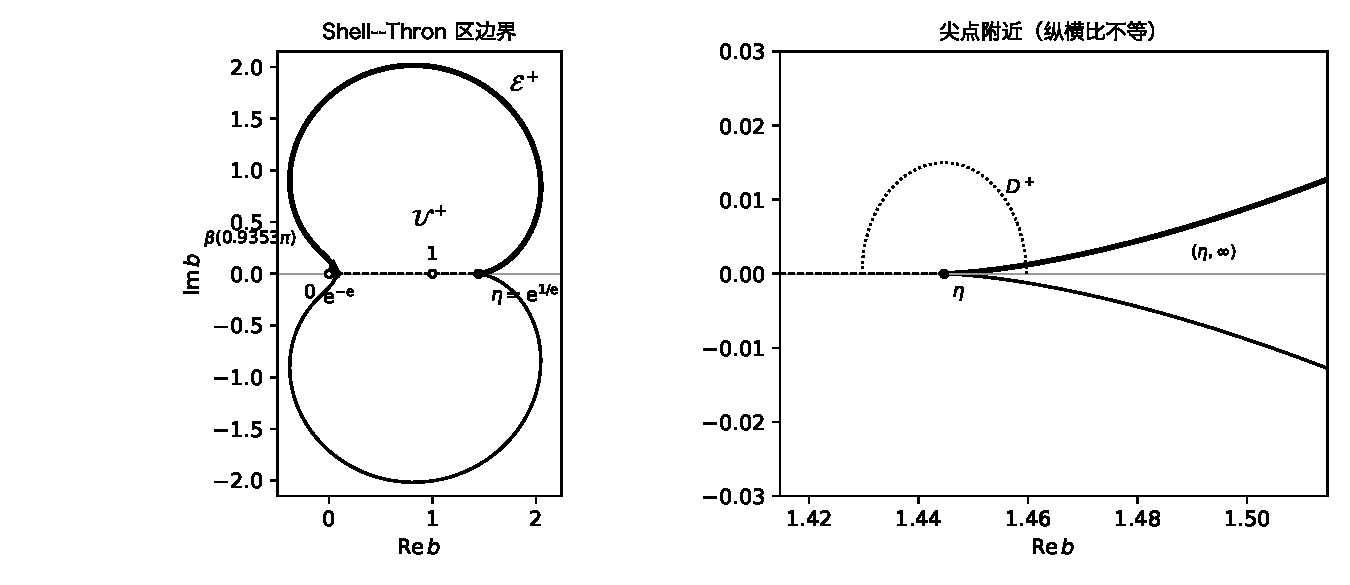
\includegraphics[width=\textwidth]{figures/fig10_shell_thron.pdf}
\caption{Shell--Thron 区的边界 $\beta(\alpha)$（粗线为上中性弧 $0<\alpha<\pi$），实段 $[\ee^{-\ee},\eta]$（虚线），
奇点 $0$、$1$（空心点），以及 \cref{ch10:thm:far-arc} 中的 $\beta(0.9353\pi)$。右图放大尖点 $\eta$ 附近，
外侧实射线 $(\eta,\infty)$ 夹在两条边界弧形成的细角中，虚线半圆是 \cref{thm:cusp} 中的 $D^+$。
脚本 \texttt{figures/fig10\_shell\_thron.py}。}
\label{ch10:fig:shell-thron}
\end{figure}

\Cref{ch10:fig:shell-thron} 中有以下几个特殊点和实段。
\begin{itemize}
\item \textbf{尖点} $\eta=\beta(0)$，乘子 $1$：鞍结点。
\item 实段 $(1,\eta)$：两个实不动点，吸引的乘子 $\lambda_1\in(0,1)$，排斥的 $\lambda_2>1$。这是第 4--9 章的 $s>0$ 一侧。
\item 外侧实射线 $(\eta,\infty)$：共轭排斥不动点对，Kneser 解所在之处。
\item 实段 $(\ee^{-\ee},1)$：吸引不动点的乘子 $\lambda\in(-1,0)$。
\item \textbf{端点} $\ee^{-\ee}=\beta(\pi)$：乘子 $-1$，倍周期分岔点。
\item 实段 $(0,\ee^{-\ee})$：吸引的二周期轨道。
\item $b=1=b(0)$：$E_1\equiv1$，乘子 $0$。它在 $\STreg$ 内部，但如下所述是 Kneser 族的奇点。
\item $b=0$：边界外的极限点，也是奇点。
\end{itemize}

\subsection{尖点}

在 $\eta$ 附近用复参数 $\varepsilon=1-\lambda_1$（本章专用，见记号表）。由 \cref{ch10:lem:param}，
\begin{equation}\label{ch10:eq:cusp-param}
  \log b(\varepsilon)=(1-\varepsilon)\ee^{\varepsilon-1},\qquad
  \log b-\log\eta=-\frac{1}{2\ee}\,\psi_0(\varepsilon)^2,\quad \psi_0(\varepsilon)=\varepsilon(1+O(\varepsilon)) .
\end{equation}
所以 $\varepsilon\mapsto b$ 在 $0$ 附近是 $2:1$ 的。三条曲线在 $\varepsilon$ 平面中的样子是：
\begin{itemize}
\item 实 $b<\eta$：$\varepsilon>0$ 实；
\item 实 $b>\eta$：$\varepsilon(\theta)=1-\theta\cot\theta-\ii\theta=\tfrac13\theta^2-\ii\theta+O(\theta^4)$，$\theta>0$ 小；
\item 上中性弧：$\varepsilon=1-\ee^{\ii\phi}=-\ii\phi+O(\phi^2)$，$\phi>0$ 小，这时 $b-\eta$ 是 $-\varepsilon^2=\phi^2+\ii\phi^3+O(\phi^4)$ 的正倍数。
\end{itemize}
因此上半圆盘 $D^+=\{|b-\eta|<r,\ \Ima b>0\}$ 连同两侧的实段，是 $\varepsilon$ 平面中一个扇形
\[
  \mathcal S_r=\Bigl\{0<|\varepsilon|<r,\ -\tfrac{7\pi}{12}<\arg\varepsilon<\tfrac{\pi}{12}\Bigr\}
\]
的像的一部分（\cite[引理~10.1]{KneserPaper}）。记 $\mathcal S'_r\subset\mathcal S_r$ 为把两条边界射线各向内收 $\tfrac1{10}$ 弧度所得的子扇形；
族建在 $\mathcal S'_r$ 上，使得下面第 6 步中参数圆盘仍留在 $\mathcal S_r$ 内。由于 $b-\eta=-\frac{\eta}{2\ee}\psi_0(\varepsilon)^2\bigl(1+O(\varepsilon^2)\bigr)$，
在 $b$ 平面中经上半圆盘从外侧实射线走到内侧实段（绕尖点转过角度 $\pi$），在 $\varepsilon$ 平面中变成在扇形中从
$\arg\varepsilon\approx-\pi/2$（外侧实射线）转到 $\arg\varepsilon=0$（内侧实段），途中经过 $\arg\varepsilon\approx-\pi/2$ 附近的中性弧。
外侧实射线与中性弧在 $\varepsilon$ 平面中只差 $O(\theta^2)$，这对应图中的细角。

\begin{example}[底数平面的几个数值]\label{ch10:ex:base-numbers}
脚本 \texttt{figures/fig10\_shell\_thron.py}（mpmath，30 位）给出
\[
\begin{gathered}
  \eta=1.44466786100976613\ldots,\qquad \ee^{-\ee}=0.0659880358453125\ldots,\\
  \beta(\tfrac\pi4)=1.63364638222+0.06303054219\,\ii,\qquad
  \beta(\tfrac\pi2)=1.98933207608+1.19328219947\,\ii,\\
  \beta(0.9353\pi)=0.04308627075+0.07503244068\,\ii .
\end{gathered}
\]
论文 11.5 节数值检验的边界点 $\alpha=2\pi(\sqrt2-1)/5$ 是 $b_c=1.52167792861+0.01481787639\,\ii$。
\Cref{ch10:sec:upper} 的直弦参数 $\theta$ 满足 $\theta\cot\theta+\ii\theta=-1$ 的根是
\[
  \theta_*=2.29857900665128663858+0.76604606099318995273\,\ii ,
\]
并且 $b(\theta_*)=\ee^{-\ee}$；
它与论文附录 A.2 的区间证书所验证的根一致。
\end{example}

\subsection{$b=1$ 与 $b=0$ 处的障碍}

\begin{proposition}[{\cite[命题~10.46]{KneserPaper}}]\label{ch10:prop:obstruction}
设 $W\subset\C$ 是连通区域，$0\in W$，$W+1\subset W$。
\begin{enumerate}
\item 不存在在 $W$ 与 $b=1$ 的某个圆盘之积上联合全纯、满足 $F(b,0)=1$ 与 $F(b,z+1)=\exp(F(b,z)\Log b)$ 的族。
\item 对任何在上半平面底数上满足同样条件、且 $b\to0$ 的族，$F(b,2)$ 不能全纯延拓过 $b=0$。
\end{enumerate}
\end{proposition}

\begin{proof}
(1) 若可以，则在 $b=1$ 处 $F(1,z+1)=1$ 对 $z\in W$ 成立。$W+1$ 是 $W$ 的非空开子集，由恒等定理 $F(1,\cdot)\equiv1$。
令 $H(z)=\partial_bF(1,z)$。对函数方程在 $b=1$ 处关于 $b$ 求导：
$\partial_bF(b,z+1)=\exp(F\Log b)\,(\partial_bF\cdot\Log b+F/b)$，在 $b=1$ 处得 $H(z+1)=F(1,z)=1$。
再用恒等定理，$H\equiv1$；但 $F(b,0)=1$ 给出 $H(0)=0$，矛盾。

(2) 由函数方程与归一化，$F(b,1)=b$，$F(b,2)=\exp(b\Log b)$。沿 $b=\ii t$，$t\downarrow0$，这个值趋于 $1$，
而它的导数 $\exp(b\Log b)(1+\Log b)$ 无界。
\end{proof}

\begin{remark}[Paulsen 的唯一性命题]\label{ch10:rem:paulsen}
\cite{Paulsen2019} 把底数延拓族定义为 Kneser 解从 $(\eta,\infty)$ 出发沿 $b$ 的解析延拓。
其命题 2 断言：在 $\Rea z>-2$ 上解析、$F(0)=1$、在 $\pm\ii\infty$ 处趋于两个不动点的解是唯一的。
按原陈述，这对每个实 $b>\eta$ 都不成立：平移 $F_k(z)=\Kkn_b(z+z_k+2)$
给出无穷多个反例~\cite[注~1.2]{KneserPaper}；这里 $z_k$ 是非实点，满足 $E_b(\Kkn_b(z_k))=2\pi\ii k/\log b$，从而 $E_b^2(\Kkn_b(z_k))=1$。Paulsen 与 Cowgill 的唯一性定理~\cite{PaulsenCowgill2017}
不受影响，因为它还要求在 $\C\setminus(-\infty,-2]$ 上解析且实对称。对复底数需要补一个选根条件；
\cref{def:class} 的缝口高度条件就是这样一个条件。
\end{remark}

% ======================================================================
\section{绕过尖点}\label{ch10:sec:cusp}

本节陈述第一个整体定理，并说明它的证明结构。记 $W_0=\{z:\operatorname{dist}(z,[0,1])<\tfrac14\}$。
在 $b<\eta$ 一侧，第 6 章的缝合解 $\Ksew_b$（\cref{thm:sewing}）对实 $b$ 有定义，并且对 $b$ 全纯地延拓到 $(1,\eta)$ 的
一个复邻域 $N_W$（\cite[命题~3.5]{KneserPaper}；$N_W$ 的宽度没有定量）。

\begin{theorem}[绕过尖点的延拓；{\cite[定理~10.14]{KneserPaper}}]\label{thm:cusp}
存在 $r_5>0$ 和开集 $\Omega\supset D^+\cup(\eta-r_5,\eta)\cup(\eta,\eta+r_5)$，其中
$D^+=\{b:|b-\eta|<r_5,\ \Ima b>0\}$，使得以下成立。
\begin{enumerate}
\item Kneser 解 $\Kkn_b$（$b\in(\eta,\eta+r_5)$）沿底数解析延拓为 $\Omega$ 上的族，它在 $\Omega\times W_0$ 上关于 $(b,z)$ 联合全纯。
  特别地，它跨过 $D^+$ 中的 Shell--Thron 边界弧，与该处中性乘子的算术性质无关。
\item 在 $(\eta-r_5,\eta)$ 上，延拓族在 $W_0$ 上等于 $\Ksew_b$。
\item 对每个 $b\in(1,\eta)$，若 $\Kkn_{b+\ii y}$ 先经 $D^+$、再在 $N_W\cap\{\Ima b>0\}$ 内延拓，
  则极限 $\lim_{y\downarrow0}\Kkn_{b+\ii y}$ 在 $z=0$ 附近存在且等于 $\Ksew_b$；由函数方程，它在 $\Ksew_b$ 的整个正则区域上等于 $\Ksew_b$。
\end{enumerate}
\end{theorem}

把 \cref{thm:cusp} 与第 6--8 章的结果合起来，得到 Kneser 解的分离系数的极限。

\begin{corollary}[{\cite[推论~10.15]{KneserPaper}}]\label{ch10:cor:separation}
对 $b\in(1,\eta)$，边界值 $\lim_{y\downarrow0}\Kkn_{b+\ii y}$ 存在且等于 $\Ksew_b$。它的分离系数满足
$c_n/\Lam^n\to B_n\ee^{2\pi\ii na}$（$b\to\eta^-$，每个 $n\ge1$），特别地 $|c_1|/\Lam\to|B_1|=0.0890584\ldots>0$。
\end{corollary}

\begin{proof}
\cref{thm:cusp} 给出边界值等于 $\Ksew_b$；再用 \cref{thm:sewing}（$|c_n/\Lam^n-\tau_n|\le C_n\Lam$）、
\cref{thm:confluence}（$\tau_n\to B_n\ee^{2\pi\ii na}$）和 \cref{prop:B1-nonzero}。
\end{proof}

这个推论是全书的出发点：数值上看到的「Kneser 解与正则解的差的第一个 Fourier 模，按 $\Lam$ 归一化后趋于常数」，
现在有了证明，并且常数被认出是 $\ee^u-1$ 的逆 horn 映射的第一个系数。

\subsection{证明的结构}

证明分七步。下表列出每一步在论文中的位置（论文第 10.1--10.8 节，约 900 行）。
\begin{center}\small
\begin{tabular}{p{2.3cm}p{8.6cm}p{3.2cm}}
\toprule
步骤 & 内容 & 论文出处\\
\midrule
1. 尖点参数 & $\varepsilon\mapsto b(\varepsilon)$ 在扇形上单射；$f_\varepsilon-\id=(u-u_1)(u-u_2)k_\varepsilon$ & 引理 10.1\\
2. 对数坐标 & $\chi=\log\frac{u-u_1}{u-u_2}$ 中一步是平移 $-\varepsilon(1+O(|u|+|\varepsilon|))$ & 引理 10.2\\
3. 倾斜初始区域 & 可容许直线 $\ell$ 与其像之间的细带；商是 $\C^*$ & 引理 10.3、10.4\\
4. 标记点 & 基点轨道第一次进入细带；倒退回 $w=1$ & 引理 10.5、10.6，定义 10.7\\
5. 换线无关 & 不同可容许直线给出同一个解 & 引理 10.8\\
6. 全纯依赖 & Beltrami 方程，\cref{thm:ahlfors-bers} & 命题 10.9\\
7. 两端 & 外端是 Kneser 的弦；内端是缝合曲面的基本域 & 命题 10.11--10.13，定理 10.14\\
\bottomrule
\end{tabular}
\end{center}

下面逐步说明。本节的常数 $C,c$ 不依赖 $\varepsilon$。

\paragraph{第 1 步：尖点参数。}
对小的复 $\varepsilon$，令 $\lambda_1=1-\varepsilon$，$\lambda_2(\varepsilon)$ 是 $\lambda\ee^{-\lambda}=\log b(\varepsilon)$ 在 $1$ 附近的另一个根，
$\lambda_2=1+\varepsilon+\tfrac23\varepsilon^2+O(\varepsilon^3)$。不动点 $u_j=\ee^{\lambda_j-1}-1$，$u_1-u_2=-2\varepsilon(1+O(\varepsilon))$。
在实 $b>\eta$ 一侧，$\lambda_2=\overline{\lambda_1}$，$u_2=\overline{u_1}$，$u_1$ 是上方的不动点 $L_+$；
在实 $b<\eta$ 一侧，$u_1<0<u_2$ 是吸引与排斥的实不动点。所以 $u_1$ 是同一个不动点沿路径的延拓：
它在外侧是排斥的，穿过中性弧后变成吸引的。由 Weierstrass 预备定理（\cref{thm:weierstrass-prep}），
\[
  f_\varepsilon(u)-u=(u-u_1)(u-u_2)\,k_\varepsilon(u),\qquad |k_\varepsilon-\tfrac12|\le\tfrac14\quad(|u|\le\tfrac12),
\]
$k_\varepsilon$ 对 $(\varepsilon,u)$ 联合全纯。

\paragraph{第 2 步：对数坐标。}
令 $q=(u-u_1)/(u-u_2)$，$\chi=\log q$。$\chi\in2\pi\ii\Z$（称为「洞」）对应 $u=\infty$。
在离洞的距离至少 $\tfrac12$ 的区域 $\mathcal G$ 上，$u(\chi)=O(|\varepsilon|)$，所以整个 $\chi$ 平面（除去洞附近）
都被压缩到 $u=0$ 的一个 $O(|\varepsilon|)$ 邻域中。在 $\chi$ 坐标中 $f_\varepsilon$ 是
\[
  f_\chi(\chi)=\chi+\Delta(\chi),\qquad \Delta=-\varepsilon(1+\vartheta),\quad |\vartheta|\le C|\varepsilon|,\quad |\partial_\chi\Delta|\le C|\varepsilon|^2
  \quad(\chi\in\mathcal G)
\]
（\cite[引理~10.2]{KneserPaper}）。也就是说，在 $\chi$ 坐标中映射几乎是平移 $-\varepsilon$，相对误差 $O(|\varepsilon|)$，
并且在两端精确地趋于 $\Log\lambda_1$ 与 $-\Log\lambda_2$。再令 $Z=A_1\chi$，$A_1=1/\Log\lambda_1=-\varepsilon^{-1}(1+O(\varepsilon))$，
则一步是 $Z\mapsto Z+1+O(|\varepsilon|)$。这是第 7 章模型时间 $\Psi_s=A_1\log(u-u_1)+A_2\log(u-u_2)$ 的复参数版本（$A_1\chi$ 是它的主部）。

\paragraph{第 3 步：倾斜初始区域。}
令 $\omega=\ee^{\ii\alpha}$，$x_0\in[-\tfrac12,\tfrac12]$，直线 $\ell=\{\ii\pi+x_0+t\omega:t\in\R\}$。称 $\ell$ 对 $\varepsilon$ \textbf{可容许}，若
\begin{equation}\label{ch10:eq:admissible}
  \cos\alpha\ge\tfrac35,\qquad -\Ima(\varepsilon\bar\omega)\ge\tfrac12|\varepsilon| .
\end{equation}
第二个条件说：一步 $\Delta\approx-\varepsilon$ 有一个确定符号的法向分量，大小在 $[\tfrac25|\varepsilon|,\tfrac65|\varepsilon|]$ 中。
于是 $\ell$ 与 $f_\chi(\ell)$ 之间是宽为 $O(|\varepsilon|)$ 的细带 $\hat H$，它在 $u$ 平面中的像 $H^\ell_\varepsilon$ 连同 $u_1,u_2$ 是一个 Jordan 区域，
由弧 $\gamma=u(\ell)$ 与 $f(\gamma)$ 围成（\cite[引理~10.3]{KneserPaper}）。这就是\textbf{倾斜初始区域}（tilted initial region）。
\begin{itemize}
\item 在外侧实射线上（$\varepsilon=\varepsilon(\theta)$），$\alpha=0$ 可容许，$\chi\in\ii\pi+\R$ 意味着 $q<0$，即 $u$ 在 $u_1$ 与 $u_2=\overline{u_1}$ 之间的线段上：
  $\gamma$ 恰是 Kneser 的弦，$H^\ell_\varepsilon$ 恰是 Kneser 的初始区域~\eqref{ch10:eq:initial-region}。
\item 在内侧实段上（$\varepsilon>0$），$\alpha=\tfrac\pi4$ 可容许，$\alpha=0$ 不可容许（$\Ima\varepsilon=0$）。
\item 沿路径取 $\alpha(\varepsilon)=\tfrac12(\arg\varepsilon+\tfrac\pi2)$，从 $0$ 连续地转到 $\tfrac\pi4$。
\end{itemize}
初始区域就是这样被「倾斜」过去的。当 $\alpha\neq0$ 时 $H^\ell_\varepsilon$ 绕着 $u_1$ 与 $u_2$ 旋转成螺线形。

把 $\gamma$ 上的点与它在 $f(\gamma)$ 上的像粘合，得到 Riemann 曲面 $\Sigma^\ell_\varepsilon$。关键估计是：

\begin{lemma}[平坦模型；{\cite[引理~10.4]{KneserPaper}}]\label{ch10:lem:flat}
设 $\ell$ 对 $\varepsilon\in\mathcal S_{r_0}$ 可容许。在 $Z$ 坐标中，直带 $\hat H_0$（$A_1\ell$ 与 $A_1\ell+1$ 之间）模去 $\zeta\sim\zeta+1$ 是 $\C/\Z$。
映射 $\mathcal H(A_1(\ii\pi+x_0+t\omega)+\mathsf r)=A_1\bigl(\ii\pi+x_0+t\omega+\mathsf r\Delta(\ii\pi+x_0+t\omega)\bigr)$（$0\le\mathsf r\le1$）
诱导拟共形同胚 $\C/\Z\to\Sigma^\ell_\varepsilon$，$|\mathcal H(\zeta)-\zeta|\le C|\varepsilon|$，Beltrami 系数 $|\upsilon_{\mathcal H}|\le C|\varepsilon|$。
因此 $\Sigma^\ell_\varepsilon\cong\C^*$，两端（$u_1$ 端与 $u_2$ 端）对应两个穿孔。
\end{lemma}

这一步解释了为什么中性乘子不构成障碍。经典的做法是用两端的 Koenigs 坐标作穿孔坐标（\cref{ch10:prop:exterior-real} 就是这样做的），
这在乘子为中性时失效：Cremer 点没有线性化，Siegel 点的线性化不提供穿孔坐标。
这里两端是穿孔这件事，是由拟共形映射保持环形端的无穷模推出的~\cite{LehtoVirtanen}，
只用到一步估计 $A_1\Delta=1+O(|\varepsilon|)$ 和横截性 $\Ima(\Log\lambda_1\bar\omega)>0$。
不需要 Brjuno 条件，也不需要 Siegel 圆盘估计。

\paragraph{第 4 步：标记点与归一化。}
基点轨道 $\ustar_n=f^n_\varepsilon(\ustar)$ 在 $\varepsilon=0$ 时沿负实轴单调趋于 $0$，$f_0^n(\ustar)=-2/n+O(\log n/n^2)$。
在 $Z$ 坐标中它每步大约前进 $1$，法向坐标严格增加；它第一次进入细带 $\hat H$ 的点 $\chi^*_{n_0}$ 称为\textbf{标记点}
（\cite[引理~10.5]{KneserPaper}）。由 \cref{ch10:lem:flat} 的定量形式（\cite[引理~10.4(2)]{KneserPaper}），在标记点附近单值化坐标与 $Z$ 相差 $O(|\varepsilon|)$；
用 $f_\varepsilon$ 的主值逆分支沿轨道倒退 $n_0$ 步回到 $\ustar$（\cite[引理~10.6]{KneserPaper}），得到在 $W_0$ 上全纯的
\textbf{归一化倾斜解} $F^\ell_\varepsilon$，$F^\ell_\varepsilon(0)=\ustar$（即 $w=1$），$F(z+1)=f_\varepsilon(F(z))$（\cite[定义~10.7]{KneserPaper}）。
物理点 $\ustar_n$ 可能多次落在螺线形的 $H^\ell_\varepsilon$ 中；只用第一次穿越。其余的穿越对应 \cref{def:class} 之后讨论的平移伪解。

\paragraph{第 5 步：换线无关。}
若 $\ell,\ell'$ 对同一个 $\varepsilon$ 可容许，则 $F^\ell_\varepsilon=F^{\ell'}_\varepsilon$（\cite[引理~10.8]{KneserPaper}）。
证明：每次作用 $f_\chi^{\pm1}$ 使相对于 $\ell'$ 的法向坐标单调变化至少 $\tfrac25|\varepsilon|$，所以 $\hat H$ 中每个点的轨道恰有一个点落在 $\hat H'$ 中；
这给出 $\Sigma^\ell\to\Sigma^{\ell'}$ 的双全纯映射，保持两端，并把标记点送到标记点。

\paragraph{第 6 步：全纯依赖。}
在 \cref{ch10:prop:exterior-real} 中，参数依赖来自 Fischer--Grauert 局部平凡性，那里需要两端有全纯的穿孔坐标。
在中性参数处没有这样的坐标，所以改用 Beltrami 方程。固定 $\varepsilon_0$ 与一条对其邻域内所有 $\varepsilon$ 都可容许的直线 $\ell$，
映射 $\mathcal J_\varepsilon=M_\varepsilon\circ M_{\varepsilon_0}^{-1}:\hat H_{\varepsilon_0}\to\hat H_\varepsilon$ 与粘合相容，其 Beltrami 系数 $\upsilon_\varepsilon$ 满足 $|\upsilon_\varepsilon|\le\tfrac1{10}$，
并且在每点对 $\varepsilon$ 全纯。由 \cref{thm:ahlfors-bers}，归一化解 $\mathcal W_\varepsilon$ 对 $\varepsilon$ 全纯；
再用一个 $\partial_{\bar\varepsilon}$ 抵消论证（内部 Schauder 估计给出所需的 $C^1$ 正则性~\cite[第~V~章]{AhlforsLectures}），
得到 $(\varepsilon,\chi)\mapsto Z_\varepsilon(\chi)$ 联合全纯，从而 $(\varepsilon,z)\mapsto F_\varepsilon(z)$ 在 $\mathcal S'_{r_3}\times W_0$ 上联合全纯
（\cite[命题~10.9]{KneserPaper}）。

\paragraph{第 7 步：走廊的两端。}
\emph{外端}（\cite[命题~10.12]{KneserPaper}）：在 $\varepsilon(\theta)$ 处取 $\ell=\ii\pi+\R$，倾斜区域就是 Kneser 的初始区域，
标记点是实轨道穿过弦的点，所以 $F_{\varepsilon(\theta)}=\Kkn_{b}$。

\emph{内端}（\cite[命题~10.13]{KneserPaper}）：在实 $\varepsilon>0$ 处取 $\alpha=\tfrac\pi4$。在 $\Sigma$ 上用第 5 章的两个正则解的逆
$r_+=R^{-1}$ 与 $r_-=S^{-1}$ 作坐标（沿轨道的 Koenigs 时间，\cite[引理~10.10]{KneserPaper}）。关键计算是虚部：
从标记点沿细带走到 $(u_1,u_2)$ 中的点 $u_m$，$\Ima\chi$ 从 $0$ 增加到 $\pi$，路径经过下半平面，于是
\[
  \Ima r_+(u_m)=A_1\pi+O(\varepsilon)=-\tfrac h2+O(\varepsilon),
\]
而由 \cref{lem:realT}，$\Ima r_+(u_m)\in-\tfrac h2+h\Z$，所以恰为 $-\tfrac h2$。
这正是 \cref{def:class} 的缝口：$r_+=T\circ r_--\ii h$。于是 $\Theta=r_\pm$ 定义了 $\Sigma$ 到缝合曲面的全纯映射，
它把两端送到两端，并且度数为 $1$，因而是双全纯的。标记点送到吸引时间 $n_0$，所以 $F_\varepsilon=\Ksew_b$。

这里倾斜方向的符号决定了缝合分支：负斜率的直线会经过 $u_1$ 上方，给出共轭分支 $\overline{\Ksew_b(\bar z)}$，
但负斜率在实 $\varepsilon>0$ 处不可容许。所以从上半圆盘绕行选出 $\Ksew_b$，从下半圆盘绕行选出它的反射。

\paragraph{收尾。}
由 \cref{ch10:eq:cusp-param}，$\varepsilon\mapsto b(\varepsilon)$ 把 $\mathcal S'_{r_3}$ 双全纯地映到含 $D^+$ 与两侧实段的开集 $\Omega$；
外端给出 (1) 中的认同，内端给出 (2)，(3) 由 $N_W$ 上缝合族的全纯性和恒等定理推出。

\begin{remark}[没有断言的内容；{\cite[注~10.16]{KneserPaper}}]\label{ch10:rem:cusp-scope}
(1) 经下半圆盘延拓得到反射分支 $\overline{\Ksew_b(\bar z)}$。两个分支在某个实高度处至少相差 $2c\Lam$（论文推论 10.49、10.51），
这是 Kneser 族绕 $\eta$ 的单值性（monodromy）。
(2) 定理断言的是 $(b,z)$ 在 $[0,1]$ 附近的全纯性，以及经函数方程到达的正则区域；
对中性参数处 $\Ima z\to\pm\infty$ 时解的行为不作任何断言。
\end{remark}

\subsection{整个上半 Shell--Thron 区}\label{ch10:sec:global}

\cref{thm:cusp} 只在尖点附近的走廊中延拓。下一步把它推到整个 $\Uup$。

\begin{proposition}[{\cite[定理~10.22]{KneserPaper}}]\label{ch10:prop:global}
从 $(\eta,\eta+r_5)$ 出发、经 $\Omega\cap\Uup$ 的 Kneser 解，沿 $\Uup$ 中的每条路径解析延拓，
得到 $z=0$ 处的芽的单值族，关于 $(b,z)$ 联合全纯。对每个 $b_0\in(1,\eta)$，沿 $\Uup$ 中任何趋于 $b_0$ 的路径，
这些芽在 $z=0$ 的某个固定圆盘上一致收敛到 $\Ksew_{b_0}$。
\end{proposition}

证明的工具是\textbf{动力学的拟共形输运}。在乘子平面中固定一个基参数 $\lambda_0$，记 $\sigma_0$ 为吸引不动点处的 Koenigs 坐标，
$\mathfrak s=\Log\lambda$，$\mathfrak s_0=\Log\lambda_0$。在吸引域 $B_0$ 上取 Beltrami 系数
\[
  \nu_\lambda=\mathsf c(\lambda)\,\frac{\sigma_0}{\overline{\sigma_0}}\,\frac{\overline{\sigma_0'}}{\sigma_0'},\qquad
  \mathsf c(\lambda)=\frac{\mathfrak s-\mathfrak s_0}{\mathfrak s+\overline{\mathfrak s_0}},\quad |\mathsf c|<1,
\]
在 $B_0$ 外取 $0$。它是 $E_0$ 不变的，并且对 $\lambda$ 全纯。由 \cref{thm:ahlfors-bers} 得到的归一化解 $\mathcal Q_\lambda$
满足 $\mathcal Q_\lambda\circ E_0=E_\lambda\circ\mathcal Q_\lambda$（\cite[命题~10.18]{KneserPaper}）：$\mathcal Q_\lambda E_0\mathcal Q_\lambda^{-1}$ 的伸缩为零，
是 $\C$ 上覆盖 $\C^*$ 的整函数，所以形如 $\ee^{Aw}$，乘子条件迫使 $A=\lambda\ee^{-\lambda}$。
把一个倾斜初始区域用 $\mathcal Q_\lambda$ 搬过去，就得到对所有 $\lambda\in\D\cap\HH$ 由同一个公式定义的族 $\Ftr$（输运族），
它自动是单值的（\cite[命题~10.19]{KneserPaper}）。剩下的工作是比较引理：在 $\lambda_0$ 附近 $\Ftr$ 与尖点族一致（\cite[引理~10.21]{KneserPaper}）。
这需要控制 $\mathcal Q_\lambda$ 在两端的提升（\cite[引理~10.20]{KneserPaper}），是这一节技术上最细的部分。

\begin{remark}[穿孔内部；{\cite[注~10.24]{KneserPaper}}]\label{ch10:rem:punctured}
上面的构造只用到 $\Rea\mathfrak s<0$，所以 $\mathfrak s\mapsto\Ftr_{\mathfrak s}$ 在整个左半平面上单值全纯。
左半平面是 $\STreg^\circ\setminus\{1\}$ 的万有覆盖。因此 Kneser 族沿 $\STreg^\circ\setminus\{1\}$ 中每条路径都可延拓，
绕 $b=1$ 的单值性作用为 $\mathfrak s\mapsto\mathfrak s+2\pi\ii$。这个单值性是否平凡，是开放问题（\cref{ch:open}）。
数值上，边界值 $\Ksew_b$ 的 $|c_1|/\Lam$ 在 $b\downarrow1$ 时停在 $0.08$ 附近（$b=1.01$ 时为 $0.0816$），而 $\Lam\to1$。
\end{remark}

% ======================================================================
\section{整个上半平面}\label{ch10:sec:upper}

\begin{theorem}[整个上半平面；计算机辅助；{\cite[主定理~E、定理~10.40]{KneserPaper}}]\label{thm:upper-half-plane}
Kneser 解 $\Kkn_b$（$b>\eta$）沿上半平面 $\HH=\{\Ima b>0\}$ 中每条路径（取主值 $\Log b$）解析延拓。
\begin{enumerate}
\item 结果是 $z=0$ 处的芽的单值族，关于 $(b,z)$ 联合全纯。在 $\Eup=\HH\setminus\overline{\STreg}$ 上它由直弦加标记点的构造给出，
  在 $\Uup$ 上由输运族 $\Ftr$ 给出，并且全纯地跨过整条开上中性弧 $\{\beta(\alpha):0<\alpha<\pi\}$。
\item 它在 $(1,\eta)$ 上的边界值是 $\Ksew_b$，与 $\HH$ 中所用的路径无关。
\item 它全纯地延拓到实段 $[\exp(-12\ee^{12}),\exp(-\tfrac15\ee^{1/5})]\approx[\ee^{-1.95\cdot10^6},0.7833]$ 的一个邻域，
  这个实段含端点 $\ee^{-\ee}$。
\item 它全纯地跨过 $(0,\eta)\setminus\{1\}$ 的每一点；$b=0$ 与 $b=1$ 是 \cref{ch10:prop:obstruction} 意义下的真奇点。
\item 若把 \cite{Paulsen2019} 的族按其定义理解为 Kneser 解沿上半平面路径（主值对数）的解析延拓，则它就是这个族。
\item 经下半平面的延拓是复共轭族。
\end{enumerate}
\end{theorem}

\paragraph{状态。}
(1)--(3)、(5) 用到区间算术证书（证·机）；(4) 中 $(1,\eta)$ 与 $(\ee^{-\ee},1)$ 的部分以及奇点的断言是纸面证明，
$(0,\ee^{-\ee})$ 的部分把纸面论证锚定在 (3) 的证书区间中的一点上。
论文中的对应：(1) 是定理 10.33、10.34、10.40 与推论 10.35；(2) 是 \cref{ch10:prop:global}；(3) 是定理 10.43；
(4) 是定理 10.45 与命题 10.46；(5) 是推论 10.41。

\subsection{直弦加标记点}

远离尖点时，两个不动点相距不小，倾斜区域的估计（以 $|\varepsilon|$ 小为前提）不再可用。
这时用回 Kneser 自己的直弦，只是参数变成复的。对复数 $\theta$，$0<\Rea\theta<\pi$，令
\[
  \mu=\theta\cot\theta,\quad \lambda_\pm=\mu\pm\ii\theta,\quad r=\ee^{\mu},\quad
  \log b=\frac{\theta\ee^{-\mu}}{\sin\theta},
\]
则 $L_\pm=r\ee^{\pm\ii\theta}$ 是 $E_b(w)=\ee^{w\log b}$ 的不动点，乘子为 $\lambda_\pm$，且 $\log b=\lambda_+\ee^{-\lambda_+}$。
实 $\theta\in(0,\pi)$ 给出外侧实射线。仿射坐标
\[
  \zeta(w)=\frac{w/r-\cos\theta}{\ii\sin\theta}
\]
把 $L_\pm$ 送到 $\pm1$，把弦送到 $[-1,1]$，并把 $E_b$ 共轭为整函数
\begin{equation}\label{ch10:eq:seam-map}
  \mathsf s_\theta(\zeta)=\frac{\ee^{\ii\theta\zeta}-\cos\theta}{\ii\sin\theta},\qquad \mathsf s_\theta(\pm1)=\pm1,\quad \mathsf s_\theta'(\pm1)=\lambda_\pm .
\end{equation}
令 $k_\theta(t)=(\mathsf s_\theta(t)-t)/(1-t^2)$，它对 $t$ 是整函数。

\begin{lemma}[月牙形；{\cite[引理~10.27、10.38]{KneserPaper}}]\label{ch10:lem:crescent}
若对 $-1<t<1$ 有
\begin{equation}\label{ch10:eq:crescent-ineq}
  \Ima k_\theta(t)<0,\qquad \Ima\bigl(\overline{\mathsf s_\theta'(t)}\,k_\theta(t)\bigr)<0,
\end{equation}
且 $\Ima\lambda_+>0>\Ima\lambda_-$，则 $A_\theta=\mathsf s_\theta([-1,1])$ 是从 $-1$ 到 $1$ 的简单弧，除端点外在开下半平面中；
$[-1,1]\cup A_\theta$ 围出 Jordan 区域 $H_\theta$；$N_\theta(t,\sigma)=t+\sigma(\mathsf s_\theta(t)-t)$ 是 $(-1,1)\times[0,1]$ 到 $H_\theta\setminus\{\pm1\}$ 的实解析微分同胚；
粘合 $t\sim\mathsf s_\theta(t)$ 得到的曲面拟共形于 $\C/\ii\Z$，Beltrami 系数对 $\theta$ 全纯，因而它双全纯于 $\C^*$。
\end{lemma}

不等式~\eqref{ch10:eq:crescent-ineq} 的第一条说像弧在弦的下方，第二条说插值 $N_\theta$ 的 Jacobian 不变号。
它们都是关于一个实变量 $t\in[-1,1]$ 和复参数 $\theta$ 的严格不等式，正适合区间算术。

\emph{标记点。}令 $w_{-1}=0$，$w_n=E_b^n(1)$（$n\ge0$），$\zeta_n=\zeta(w_n)$。若 $w_{-1},\dots,w_{n-1}$ 都在弦的上方（$\Ima\zeta>0$），
而 $\zeta_n\in H_\theta\setminus A_\theta$，称 $n$ 为\textbf{进入指标}，$\zeta_n$ 在商曲面中的类为\textbf{标记点}。它是内蕴定义的。
单值化把两端送到 $0,\infty$、标记点送到 $1$，取对数提升并用 $E_b^{-n}$ 沿轨道倒退到 $w_0=1$，得到解 $F^{\mathrm{far}}_\theta$（\cite[定义~10.30]{KneserPaper}）。
对实 $\theta$ 它就是 Kneser 解（\cite[命题~10.32]{KneserPaper}），对 $\theta$ 联合全纯（\cite[命题~10.31]{KneserPaper}）。

于是证明整体结果的任务化为：在所需的参数集上，验证~\eqref{ch10:eq:crescent-ineq} 并找到进入指标。

\begin{theorem}[远离尖点跨过边界；{\cite[定理~10.33、10.34，推论~10.35]{KneserPaper}}]\label{ch10:thm:far-arc}
Kneser 族沿外侧路径到达上中性弧的每一点 $\beta(\alpha)$（$0<\alpha<\pi$），在 $\beta(\alpha)$ 的完整邻域上全纯，
并以芽 $\Ftr$ 进入 $\Uup$。对 $\alpha\le0.9353\ldots\pi$ 用参数区域上的证书 \texttt{certify\_far\_collar.py}，
对 $0.935\pi\le\alpha<\pi$ 用 \texttt{certify\_last\_boundary\_arc.py}。端点 $\beta(\pi)=\ee^{-\ee}$ 单独处理。
\end{theorem}

\subsection{外部区域}

在 $\Eup$ 上所有不动点都排斥，$\Eup$ 单连通，从外侧实射线延拓来的不动点 $L_+$ 单值，
其乘子 $\lambda(b)$ 把 $\Eup$ 双全纯地映到一个区域 $\mathcal V$，逆为 $\lambda\mapsto\exp(\lambda\ee^{-\lambda})$（\cite[引理~10.37]{KneserPaper}）。
对 $\lambda\in\mathcal V$，令 $\theta(\lambda)\neq0$ 是 $(\lambda-2\ii\theta)\ee^{2\ii\theta}=\lambda$ 的根；这等价于 $\lambda_+(\theta)=\lambda$，
而 $\lambda-2\ii\theta$ 是另一个不动点 $L_-=\ee^{\lambda-2\ii\theta}$ 的乘子。于是直弦构造对每个 $b\in\Eup$ 都有定义，
问题只是 $\theta(\lambda)$ 能否连续选取、以及月牙不等式与进入指标是否处处成立。
论文的命题 10.39 用一个证书回答了这个问题。

\subsection{区间证书检查什么}\label{ch10:sec:certificates}

全部证书都是用 python-flint/Arb~\cite{Johansson2017Arb} 球算术写的 Python 程序，外向舍入，每个严格不等式都在包络上判定；浮点只用来选 Krawczyk 盒的中心。
Krawczyk~\cite{Krawczyk1969} 算子
\[
  K=m-Yf(m)+\bigl(1-Yf'(B)\bigr)(B-m),\qquad K\subset\operatorname{int}B
\]
证明 $f$ 在盒 $B$ 中对给定球中的每个参数都有唯一零点（判据的陈述与证明梗概见 \cref{app:tools}）。各证书的内容如下（论文附录 A）。
\begin{itemize}
\item \texttt{certify\_far\_collar.py}（A.1，约 6 分钟，33\,027 个盒）。参数区域 $\Theta=\Theta_{\mathrm C}\cup\Theta_{\mathrm K}$ 由尖点处的锥和一块弯曲区域组成。
  在其上验证~\eqref{ch10:eq:crescent-ineq}、$|\lambda_+|$ 沿竖直纤维单调减并在顶边小于 $1$（所以每条竖直路径恰好穿过中性弧一次）、
  以及沿轨道的进入指标：要么 Krawczyk 检验证明 $\zeta_n=N_\theta(t,\sigma)$，$|t|<1$，$0<\sigma<1$；要么 $\zeta_n$ 落在一个矩形中，
  该矩形的下半部分与 $\mathsf s_\theta$ 作用后的上半部分都被证明在 $H_\theta$ 中。在锥上用解析估计代替逐盒验证（\cite[引理~10.28]{KneserPaper}）。
\item \texttt{certify\_last\_boundary\_arc.py}（A.2）。验证 $\lambda_+(\theta)=-1$ 的简单根 $\theta_*$（\cref{ch10:ex:base-numbers}）；
  在矩形 $[2.19,2.31]+\ii[0.71,0.78]$ 上验证 $\Rea(\lambda_+'(\theta)/\lambda_+'(\theta_*))>\tfrac45$，由 Noshiro--Warschawski 判据（\cref{app:tools}）
  $\lambda_+$ 在其上单射；用压缩盒得到逆分支 $\theta(\alpha)$。月牙不等式在 $[-1,\tfrac{19}{20}]$ 上直接验证，在 $[\tfrac{19}{20},1]$ 上验证导数为正，
  并用端点处的精确恒等式 $f_1(1)=f_2(1)=-\tfrac12\sin\alpha$ 闭合到 $t=1$。进入指标恒为 $-1$：$\zeta(0)=\ii\cot\theta\in\operatorname{int}H_\theta$。
\item \texttt{certify\_upper\_halfplane.py}（A.3，约 15 分钟）。四部分：(T) 尾部 $\Rea\lambda\le-12$，用 $\mathsf w=1/\lambda$ 的压缩映射定根，6\,230 个盒；
  (K) 核心 $-12\le\Rea\lambda\le5$，$|\lambda-1|\ge0.08$，丢弃确定不在 $\mathcal V$ 中的盒（用 $\phi(\D)$ 的星形边界），在其余盒上用 Krawczyk 定根，
  相邻盒的根用凸包上的唯一性对接；(P) 尖点 $|\lambda-1|<0.08$，用 Rouché 定理（\cref{app:tools}）证明根唯一并落在锥 $\Theta_{\mathrm C}$ 中；
  (I) 接口与锚点：在 $\lambda=\cot1+\ii$ 处的盒包含实根 $\theta=1$，这把整条分支锚定在外侧实射线上。
\item \texttt{certify\_endpoint.py}（A.4，不到 1 分钟）。在 $\ee^{-\ee}$ 附近与实段上，直弦构造在一个对数坐标中验证（论文引理 10.42 的条件 (a)--(f)）。
\end{itemize}
外侧覆盖、尖点与接口合起来证明：$\theta(\lambda)$ 在 $\mathcal V$ 上是一条连续分支，处处满足月牙条件并有进入指标。
再加上 \cref{ch10:thm:far-arc} 和 \cref{ch10:prop:global}，三块（$\Eup$、开中性弧、$\Uup$）在重叠处一致，
$\HH$ 单连通，所以延拓与路径无关。这就是 \cref{thm:upper-half-plane}(1)(2)。

\subsection{端点与 $\eta$ 以下的实轴}

\emph{端点。}在 $\ee^{-\ee}$ 附近，伙伴不动点 $L_-$ 不是实的，构造不对共轭对称，所以经上半平面与经下半平面的延拓不必一致。
直弦构造在乘子平面的正方形 $[-1.1,-0.9]\times[-0.1,0.1]$ 和长条 $[-12,-\tfrac15]\times[-10^{-3},10^{-3}]$ 上被验证，标记点为 $w_{-1}=0$
（\cite[定理~10.43]{KneserPaper}）。

\emph{二周期段。}对 $b=\ee^{-\mathcal M}\in(0,\ee^{-\ee})$，实二周期轨道 $p<q$ 的乘子 $m$ 有显式参数化
\[
  \mathcal Mp=u(\coth u-1),\quad \mathcal Mq=u(\coth u+1),\quad \mathcal M=\frac{u}{\sinh u}\ee^{u\coth u},\quad m=\Bigl(\frac{u}{\sinh u}\Bigr)^2,\quad u>0,
\]
$\mathcal M$ 从 $\ee$ 增到 $\infty$，$m$ 从 $1$ 减到 $0$。所以 $m$ 是整段 $(0,\ee^{-\ee})$ 上的实解析坐标。
以二周期的 Koenigs 坐标作输运（与 \cref{ch10:sec:global} 相同的拟共形技术），锚定在证书区间中的 $b_*=\exp(-2\ee^2)$ 处
（\cite[定理~10.45]{KneserPaper}）。

\emph{实段 $(1,\eta)$ 与 $(\ee^{-\ee},1)$。}前者由 \cref{ch10:prop:global} 与缝合族的参数全纯性得到，后者由输运族直接跨过（\cite[命题~10.23]{KneserPaper}）。

\begin{remark}[与 Paulsen 族的关系]\label{ch10:rem:paulsen-family}
\cite{Paulsen2019} 的族由底数上的解析延拓定义，但那里跨过 Shell--Thron 边界只有数值论证（数值格式的连续性）。
\cref{thm:upper-half-plane}(5) 解决了这一点。在 $b=\sqrt2$ 处，缝合方程给出 $\Ima\Ksew_{\sqrt2}(\tfrac12)=-1.18899697185\cdot10^{-48}$，
与 Paulsen 的 120 位计算值 $-1.18899697\cdot10^{-48}$ 在给出的全部 9 位（含符号）上一致~\cite[第~11~节]{KneserPaper}。
这是数值核对，不是证明的一部分。
\end{remark}

% ======================================================================
\section{其他族}\label{ch10:sec:other}

一般理论对下面三个族逐字成立：只需验证 (H1)--(H4)，并对需要 (H5) 的陈述单独处理 $B_1\neq0$。
整体结果（\cref{thm:cusp}、\cref{thm:upper-half-plane} 的类比）则依赖每个族的整体几何。

\subsection{三个族的开折数据}

\begin{example}[$w^2+c$]\label{ch10:ex:quad}
$f_c(w)=w^2+c$ 在 $c=\tfrac14$ 处有二重不动点 $w^*=\tfrac12$。令 $c=\tfrac14-s$，$u=w-\tfrac12$，
则 $f_s(u)=u+u^2-s$：$g(u)=u+u^2$，$a_2=1$，$a_3=0$，$\rho=1$，$X=1$，$\gamma=1$。这是平移开折，所以 $\kappa^{(n)}=\ktr^{(n)}(u+u^2)$。
$s>0$ 时有两个实不动点 $\tfrac12\pm\sqrt s$。基点可取 $w_0=0$、$0.2$、$0.35$ 或 $f_c^3(0)$（在 $c=\tfrac14$ 处为 $\tfrac{89}{256}$）；
它们都满足 (H4)。$B_1\neq0$：直接吸引域中只有一个临界点（\cite[注~9.5]{KneserPaper}）。
\end{example}

\begin{example}[$v-\sin v+c$]\label{ch10:ex:sine}
$f_c(v)=v-\sin v+c$ 的二重不动点要求 $\sin v=c$，$\cos v=0$，取 $v^*=\tfrac\pi2$，$c=1$。令 $c=1-s$，$u=v-\tfrac\pi2$，
则 $f_s(u)=u+1-\cos u-s$：$g(u)=u+\tfrac12u^2-\tfrac1{24}u^4+\cdots$，$a_2=\tfrac12$，$a_3=0$，$\rho=1$，$X=1$，$\gamma=1$。
临界值 $2\pi k+1$ 都是实的，直接吸引域只含 $k=0$ 那一个；但 $f$ 有无穷多个临界值，不是有限型，Chéritat 的单奇值论证能否适用需要核查。
所以 $B_1\neq0$ 的状态是「推导」，(H5) 作为假设保留。
\end{example}

\begin{example}[$w+(w^2-c)\ee^w$]\label{ch10:ex:expq}
$f_c(w)=w+(w^2-c)\ee^w$ 在 $c=0$ 处有二重不动点 $w^*=0$。令 $c=s$，则 $f_s(u)=u+u^2\ee^u-s\ee^u$：
$g(u)=u+u^2+u^3+\cdots$，$a_2=1$，$a_3=1$，$\rho=0$，$X=\ee^u$，$\gamma=1$。$s>0$ 时不动点是 $\pm\sqrt s$，两个乘子 $1\pm2\sqrt s\,\ee^{\pm\sqrt s}$ 不对称。
$B_1\neq0$ 只有数值（$|B_1|\approx2744$）。
\end{example}

\begin{example}[数值比较]\label{ch10:ex:numerics-table}
脚本 \texttt{generality\_check.py}（论文注 9.14）对任意给定 $f$ 及其在不动点处的 Taylor 系数实现第 5--8 章的构造。
下表是 $\lambda_1=0.97$ 处的值（取自 $\lambda_1=0.5,\dots,0.97$ 的扫描）；第四列在 $p\to0$ 时趋于 $\Rea\kappa^{(1)}$。
\begin{center}\small
\begin{tabular}{lllll}
\toprule
族 & $\rho$ & $|B_1|$ & $\Rea\log(\tau_1/B_1\ee^{2\pi\ii a})/p$ & $|\tau_1|/|B_1|-1$\\
\midrule
$b^w$ & $1/3$ & $0.0890584364122$ & $-0.0101990$ & $-9.4\cdot10^{-6}$\\
$w^2+c$ & $1$ & $0.0597942361690$ & $-0.0150481$ & $-1.4\cdot10^{-5}$\\
$v-\sin v+c$ & $1$ & $0.0723786416245$ & $-0.0142133$ & $-1.3\cdot10^{-5}$\\
$w+(w^2-c)\ee^w$ & $0$ & $2744.09379131$ & $+1.08542$ & $+1.0\cdot10^{-3}$\\
\bottomrule
\end{tabular}
\end{center}
在每个族中，$\tau_n$、$t_n/t_1^n$ 与 $\log(\tau_1/B_1\ee^{2\pi\ii a})/p$ 都以 $O(p)$ 的速率收敛；缝口条件 $\Ima t_0=h/2$ 精确到 $10^{-31}$ 以上；
缝合迭代给出 $\hat c_n=\tau_n(1+O(\Lam))$。对 $w^2+c$ 用三个基点 $w_0=0,0.2,0.35$，第四列的实部在显示的 10 位上一致（\cref{prop:base-point}），
虚部则从 $-0.07$ 变到 $116$。$w^2+c$ 的极限值是 $\Rea\ktr^{(1)}(u+u^2)=-0.0150441028391897$（\texttt{kappa\_variation.py}）。
$w^2+c$ 与 $v-\sin v+c$ 的芽有相同的 $\rho$，因而形式共轭，但 $|B_1|$ 不同（数值），所以它们不是实解析共轭的（\cref{cor:invariance}）。
\end{example}

\paragraph{状态。}三个新族上，汇流、缝合解、一阶与全阶展开、基点无关性都是一般定理的特例（已证）；
$B_1\neq0$ 对 $w^2+c$ 已证，对 $v-\sin v+c$ 是推导，对 $w+(w^2-c)\ee^w$ 是数值。
整体延拓：$w^2+c$ 见下一小节；另外两个族\textbf{未检验}。

\subsection{$w^2+c$ 的整体延拓}

对应关系如下。实 $c>\tfrac14$ 时两个不动点 $\tfrac12\pm\ii\sqrt{c-\tfrac14}$ 共轭排斥，实轴逃逸；Shell--Thron 区对应 Mandelbrot 集的主心形区
$\mathcal C=\{\lambda/2-\lambda^2/4:|\lambda|<1\}$；尖点 $\eta$ 对应 $c=\tfrac14$；端点 $\ee^{-\ee}$ 对应 $c=-\tfrac34$（乘子 $-1$）。
归一化取 $F_c(0)=f_c^3(0)$，对应以临界点为标记 $F(-3)=0$。

这个族的直弦几何是精确的，不需要区间算术。设 $c\in\HH$，取全纯平方根 $a(c)$，$a^2=\tfrac14-c$，$\Rea a<0<\Ima a$。
在坐标 $w=\tfrac12+a\zeta$ 中，不动点 $\tfrac12\pm a$ 对应 $\zeta=\pm1$，映射变为
\[
  S_a(\zeta)=\zeta+a(\zeta^2-1).
\]

\begin{proposition}[二次族的直月牙；\texttt{docs/proofs/quadratic-continuation.tex} 定理 1]\label{ch10:prop:quad-crescent}
对每个 $c\in\HH$，弦 $[-1,1]$ 与它的像 $S_a([-1,1])$ 只在端点相交，围出 Jordan 区域 $H_a$，参数化为
$M_a(t,\sigma)=t+\sigma a(t^2-1)$，$-1\le t\le1$，$0\le\sigma\le1$。开区域是凸的，含于 $\Ima\zeta<0$，并且 $S_a$ 在整个下半平面上单射。
\end{proposition}

\begin{proof}
写 $a=r+\ii\beta$，$\beta>0$，引入实线性坐标 $T=\Rea\zeta-(r/\beta)\Ima\zeta$，$Y=\Ima\zeta/\beta$。
对 $\zeta=M_a(t,\sigma)$ 有 $T=t$，$Y=\sigma(t^2-1)$。所以开区域恰是 $\{-1<T<1,\ T^2-1<Y<0\}$，
它是凸函数 $T^2-1$ 的上图与一个半平面之交在可逆线性映射下的像，因而是凸的；两条边界弧的 $T$ 坐标都是 $t$，$Y$ 坐标分别是 $0$ 与 $t^2-1$，
所以它们单射且内部不交。若 $S_a(\zeta)=S_a(\zeta')$，$\zeta\neq\zeta'$，则 $\zeta+\zeta'=-1/a$，其虚部为正；
所以闭下半平面中两点不会碰撞。
\end{proof}

在此基础上，证明稿（\texttt{docs/proofs/quadratic-continuation.tex}，2026-10-04）给出了论文主定理 D、E 的二次族类比的证明：
\begin{itemize}
\item \textbf{二次族 G}（证明稿定理 16，\texttt{thm:G}）：$c>\tfrac14$ 的临界轨道标记的实 Kneser 月牙族在整个 $\HH$ 上有单值全纯延拓，
  在每个 $c_0\in\HH$ 附近由联合全纯的 $F(c,z)$ 表示，$F(c,0)=f_c^3(0)$。
\item \textbf{二次族 F}（证明稿定理 20，\texttt{thm:F}）：该族经 $c=\tfrac14$ 的上方穿孔邻域延拓，跨过中性边界而不需要乘子的算术条件；
  它在每个实 $0<c<\tfrac14$ 处的边界值是由接缝 $T-\ii h$ 指定的缝合解 $\Ksew_c$；它在整个上主心形区中单值。
\end{itemize}
证明的组成：直月牙几何（\cref{ch10:prop:quad-crescent}）；对 $|a|>\tfrac12$，临界值 $c$ 严格位于月牙内部，用作标记（习题~\ref{ch10:ex:quad-mark}）；
$0<|a|\le\tfrac1{16}$ 用解析的首次穿越估计；其余的紧区域 $\tfrac1{16}\le|a|\le\tfrac12$ 用 4\,013 个闭参数盒的 Arb 覆盖
（\texttt{certify\_quad\_entry.py}，最大轨道指标 21），并由独立程序 \texttt{verify\_quad\_entry.py} 以 90 位精度重放、用 282 个有理横向分片验证精确覆盖；
主心形区内用显式的多项式乘子形变输运（从 $\lambda_*=\ii/2$ 出发，主解为奇函数、保持临界点 $0$），并在开重叠集上与直弦族比较；
尖点走廊用倾斜区域，常数由 \texttt{certify\_quad\_geometry.py} 的 14 项 Arb 检查核验。

\paragraph{状态与范围。}二次族 F、G 是\textbf{单独的证明稿}中的结果（作者标为已证 + 证·机），不在投稿论文中，也不由一般理论推出。
证明稿是 2026-10-04 的研究笔记，\textbf{未经同行评审}；本书只转述其结构，不对其正确性背书。
它们用到了二次多项式特有的结构（精确月牙、临界点标记、主心形区的显式输运）。
证明稿不断言在尖点本身、实端点 $c=-\tfrac34$ 处的延拓，也不断言所有参数有一个共同的整体高度定义域。
此前的数值证据（$\theta$ 迭代在 $c$ 平面采样点上的收敛、跨中性带插值、竖直阶梯外推 $\hat c_1$ 与 $\tau_1$ 吻合到 $O(\Lam)$ 修正项本身的 0.3\%）
只是数值，它们并不蕴含证明，证明也不蕴含该数值算法的收敛。

\begin{example}[$\theta$ 迭代的共振障碍]\label{ch10:ex:theta-obstruction}
用两侧 Schröder（Koenigs）表示求值的 $\theta$ 迭代算法，不能在整个 $\HH$ 上收敛。取 $c=\tfrac14+\tfrac\ii2$，
上方不动点 $L=\tfrac\ii2$，乘子 $\lambda=2L=\ii$。逆 Schröder 级数 $u(\zeta)=\sum_{k\ge1}u_k\zeta^k$，$u(\lambda\zeta)=\lambda u(\zeta)+u(\zeta)^2$，
要求
\[
  (\ii^k-\ii)\,u_k=\sum_{j=1}^{k-1}u_ju_{k-j},\qquad u_1=1 .
\]
逐阶解出 $u_2=\tfrac{-1+\ii}2$，$u_3=\tfrac{-1-\ii}2$，$u_4=\tfrac{1-5\ii}4$；到 $k=5$ 左边系数 $\ii^5-\ii=0$，右边却是 $\tfrac{3-5\ii}2\neq0$。
所以形式级数都不存在。更一般地，若 $w^2+c$ 的不动点乘子 $\lambda$ 是 $q$ 次单位根且可线性化，则 $f_c^q$ 在该点附近共轭于恒等映射，
从而 $f_c^q=\id$，与 $\deg f_c^q=2^q$ 矛盾。这样的参数在开中性弧上稠密。
精确有理数验证见 \texttt{certify\_quad\_theta\_obstruction.py}（9 项检查）。这个反例\textbf{不}否定二次族 F、G：
商曲面的构造不需要固定点的线性化（与 \cref{ch10:lem:flat} 后的讨论相同）。
\end{example}

\subsection{什么是一般的，什么是特殊的}

\begin{center}\small
\begin{tabular}{p{4.2cm}p{4.6cm}p{4.2cm}}
\toprule
结果 & 用到族的什么 & 状态\\
\midrule
转移映射、焊接恒等式、缝合解 & 两个实双曲不动点及其间的不变区间 & 一般（已证）\\
汇流、一阶与全阶展开、变分公式 & 抛物芽与开折方向 & 一般（已证）；需 (H5) 的部分见上\\
$B_1\neq0$ & 直接吸引域中只有一个奇异值 & exp、quad 已证；sine 推导；expq 数值\\
绕尖点（\cref{thm:cusp}） & 尖点处二次切；指数族的具体估计 & tetration 已证；quad 单独证明稿（未审稿）；其他未检验\\
全上半平面（\cref{thm:upper-half-plane}） & 指数函数的整体几何 & tetration 证·机；quad 单独证明稿（未审稿）；其他未检验\\
\bottomrule
\end{tabular}
\end{center}
绕尖点的论证只用到尖点附近的局部估计（第 1--6 步）和内端的缝合认同（第 7 步），后者是一般理论的一部分；
外端用到的是「外侧实参数处有一个 Kneser 型构造」。所以 \cref{thm:cusp} 移植到一般开折的障碍主要在外端：
一般的族在尖点的另一侧不一定有共轭不动点对的实构造。这个问题在 \cref{ch:open} 中作为 C3 讨论。

% ======================================================================
\notes

\paragraph{Kneser 与 Shell--Thron。}Kneser 的构造见~\cite{Kneser1950}；其初始区域的表述与唯一性刻画见 Trappmann 与 Kouznetsov~\cite{TrappmannKouznetsov2011}，
高精度算法见~\cite{Kouznetsov2009,KouznetsovTrappmann2010,KouznetsovTrappmann2012}。
Shell--Thron 区得名于 Thron~\cite{Thron1957} 与 Shell~\cite{Shell1962} 关于无穷幂塔收敛的工作。
Paulsen~\cite{Paulsen2019} 提出沿底数延拓 Kneser 解，\cite{PaulsenCowgill2017} 给出实底数 $b>\eta$ 时的唯一性定理，
\cite{Paulsen2026} 研究了 $b\to1$ 时部分非整数高度的行为。Nixon~\cite{Nixon2022} 用无穷复合构造 Shell--Thron 区内部的非正则解，
并用 1-周期的 $\theta$ 映射与正则解比较；这正是本书的分离形式 $K=R\circ(\id+P)$。

\paragraph{与论文的对应。}本章的 \cref{thm:cusp} 是论文主定理 D 的精确形式（论文定理 10.14，标签 \texttt{thm:cusp}）；
\cref{ch10:prop:global} 是论文定理 10.22（\texttt{thm:global}），与定理 10.14 合起来给出主定理 D；\cref{thm:upper-half-plane} 汇总论文主定理 E，
其精确形式分布在定理 10.33（\texttt{thm:far}）、10.34（\texttt{thm:last-arc}）、10.40（\texttt{thm:upper}）、10.43（\texttt{thm:endpoint}）、
10.45（\texttt{thm:positive-real-axis}）、命题 10.46（\texttt{prop:zero-one-obstruction}）与推论 10.41（\texttt{cor:paulsen}）中。
区间证书的说明在论文附录 A.1--A.5。论文的引理编号以 2026-10-07 的 \texttt{main.pdf} 为准。

\paragraph{一般族。}三个新族的数值检验与假设审查见论文第 9 节（注 9.5、9.13、9.14、9.15）。
二次族 F、G 的证明稿 \texttt{docs/proofs/quadratic-continuation.tex} 还包含一个一般的「带标记柱面延拓判据」和一个单位根共振障碍的一般形式，
它们指出了把 F、G 推广到二次以外所需的额外假设（\cref{ch:open}）。

\paragraph{形式化。}Lean 4 工程对 tetration 形式化了缝合、汇流基线与全阶展开；\cref{thm:cusp} 与 \cref{thm:upper-half-plane} \textbf{没有}形式化。

% ======================================================================
\exercises

\begin{exercise}\label{ch10:ex:data}
验证 \cref{ch10:prop:data}：对 $f_s(u)=\ee^{u-s(1+u)}-1$ 计算 $a_2,a_3,\rho$、$X$ 与 $\gamma$，并验证恒等式~\eqref{ch10:eq:cohomologous}。
\end{exercise}

\begin{exercise}\label{ch10:ex:p}
设 $\lambda_1=1-\varepsilon$，$\lambda_2$ 是 $\lambda\ee^{-\lambda}=\lambda_1\ee^{-\lambda_1}$ 的另一个根。
(1) 证明 $\lambda_2=1+\varepsilon+\tfrac23\varepsilon^2+O(\varepsilon^3)$。
(2) 证明 $s=1-(1-\varepsilon)\ee^{\varepsilon}=\tfrac12\varepsilon^2+\tfrac13\varepsilon^3+O(\varepsilon^4)$。
(3) 由此证明 $p=-\log\lambda_1\log\lambda_2=2s+\tfrac{10}9s^2+O(s^3)$。
\end{exercise}
\begin{hint}
(1) 令 $\lambda_2=1+\delta$，比较 $\ee^{-1}(1-\tfrac12\delta^2+\tfrac13\delta^3)$ 与 $\ee^{-1}(1-\tfrac12\varepsilon^2-\tfrac13\varepsilon^3)$。
(3) 先把 $p$ 展开到 $\varepsilon^4$，再用 (2) 反解 $\varepsilon$。
\end{hint}

\begin{exercise}\label{ch10:ex:exterior}
设 $b>\eta$ 实，$L_+$ 是主不动点，$\theta=\Ima(L_+\log b)\in(0,\pi)$。
(1) 证明乘子 $\lambda_+=L_+\log b=\theta\cot\theta+\ii\theta$，从而 $|\lambda_+|=\theta/\sin\theta>1$。
(2) 证明 $E_b$ 把竖直弦 $\gamma_b$ 映成以 $0$ 为心、半径 $|L_+|$ 的圆弧。
\end{exercise}
\begin{hint}
(1) 由 $L=\ee^\lambda$ 与 $\log b=\lambda\ee^{-\lambda}$ 实，得 $\Ima(\lambda\ee^{-\lambda})=0$，即 $\ee^{-\Rea\lambda}(\theta\cos\theta-\Rea\lambda\sin\theta)=0$。
\end{hint}

\begin{exercise}\label{ch10:ex:two-cycle}
设 $\mathcal M>\ee$，$E(w)=\ee^{-\mathcal Mw}$。对 $u>0$ 令 $\mathcal Mp=u(\coth u-1)$，$\mathcal Mq=u(\coth u+1)$。
证明当 $\mathcal M=\frac{u}{\sinh u}\ee^{u\coth u}$ 时 $\{p,q\}$ 是 $E$ 的二周期轨道，乘子为 $(u/\sinh u)^2$；并证明 $\mathcal M$ 关于 $u$ 递增、乘子递减。
\end{exercise}

\begin{exercise}\label{ch10:ex:obstruction}
补全 \cref{ch10:prop:obstruction}(1) 的证明中关于 $b$ 求导的一步，并说明为什么需要 $W+1\subset W$ 且 $W$ 连通。
(2) 中为什么沿 $b=\ii t$ 而不是沿实轴取极限？
\end{exercise}

\begin{exercise}\label{ch10:ex:admissible}
(1) 证明对 $\varepsilon\in\mathcal S_r$，$\alpha(\varepsilon)=\tfrac12(\arg\varepsilon+\tfrac\pi2)$ 满足可容许条件~\eqref{ch10:eq:admissible}。
(2) 证明在实 $\varepsilon>0$ 处，$\alpha=0$ 不可容许，任何 $\alpha<0$ 也不可容许。
(3) 结合 \cref{ch10:sec:cusp} 第 7 步，说明为什么经上半圆盘绕行选出的是 $\Ksew_b$ 而不是 $\overline{\Ksew_b(\bar z)}$。
\end{exercise}

\begin{exercise}\label{ch10:ex:quad-mark}
在 \cref{ch10:prop:quad-crescent} 的坐标中，设 $R=|a|>\tfrac12$。证明临界值 $w=c$ 的坐标为
$T(c)=-r/(2R^2)$，$Y(c)=-1+1/(4R^2)$，并且 $Y(c)-(T(c)^2-1)=\beta^2/(4R^4)>0$，所以 $c$ 严格在月牙内部。
\end{exercise}
\begin{hint}
$c=\tfrac14-a^2$，$\zeta(c)=(c-\tfrac12)/a=-(a^2+\tfrac14)/a$。
\end{hint}

\begin{exercise}\label{ch10:ex:quad-resonance}
(1) 用精确有理数算术复核 \cref{ch10:ex:theta-obstruction} 中的 $u_2,\dots,u_4$ 与 $k=5$ 处的矛盾。
(2) 证明：若一个多项式 $P$（$\deg P\ge2$）在不动点处的乘子是 $q$ 次本原单位根并且可线性化，则 $P^q=\id$，矛盾。
(3) 为什么这个障碍不影响 \cref{ch10:lem:flat} 那样的商曲面构造？
\end{exercise}

\begin{exercise}\label{ch10:ex:formal}
(1) 证明 $u+u^2$ 与 $u+\tfrac12u^2-\tfrac1{24}u^4$ 在 $u\mapsto cu$（$c>0$）的伸缩下可以化为相同的 $a_2$，并且二者的迭代留数都是 $1$。
(2) 证明在实伸缩 $u\mapsto cu$ 下，$\alpha$ 的归一化只改变一个实常数，因此 $|B_n|$ 不变。
(3) 利用 \cref{ch10:ex:numerics-table} 的数值，说明这两个芽形式共轭但（在数值准确的前提下）不实解析共轭。
\end{exercise}

\begin{exercise}\label{ch10:ex:generalize}
（研究性）设一个实鞍结开折在参数 $s<0$ 一侧有一对共轭排斥不动点，并且在其间有一个 Kneser 型初始区域。
列出把 \cref{thm:cusp} 的第 1--7 步移植到这个开折所需的全部输入。哪些是局部的（只依赖尖点附近），哪些是整体的？
\end{exercise}
\begin{hint}
第 1--6 步只用到 Weierstrass 预备与一步估计；第 7 步内端用到 \cref{thm:characterization}，外端需要一个已知的外侧构造及其实参数解析性（\cref{ch10:prop:exterior-real}）。
\end{hint}
